\section{Altium Designer}
\subsection{Button Input}

Push buttons or switches connect two points in a circuit when you press them. Inasystem,
button is a traditional input method.
\subsubsection{Schematic design}
\textbf{Your image goes here:}
\begin{figure}[h!]
    \centering
    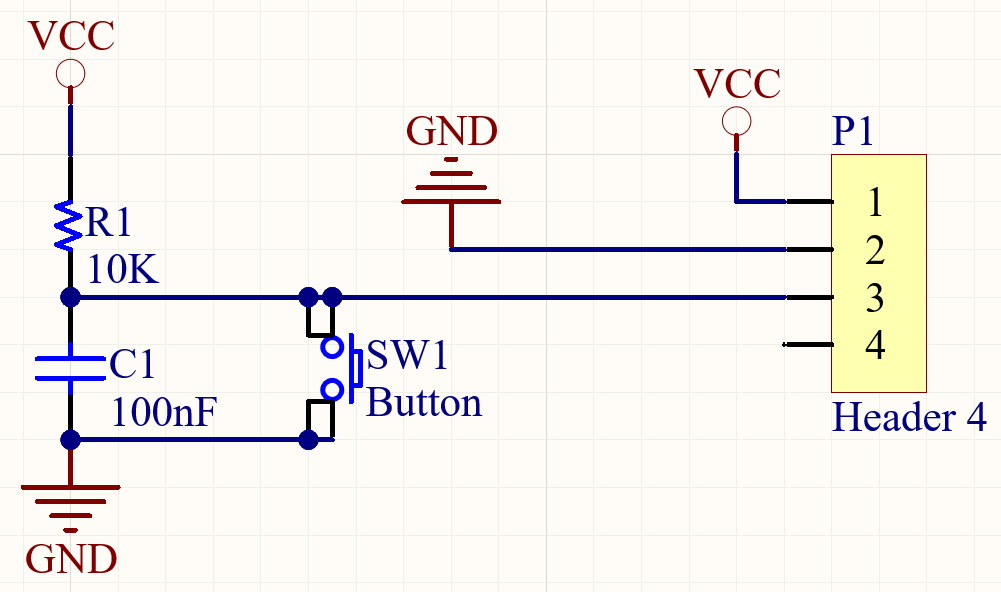
\includegraphics[width=0.7\textwidth]{graphics/ex4/f1.png}
\end{figure}

\subsubsection{PCB layout}
\textbf{Your images go here:}
\begin{figure}[h!]
    \centering
    % Ảnh trái
    \begin{subfigure}{0.495\textwidth}
        \centering
        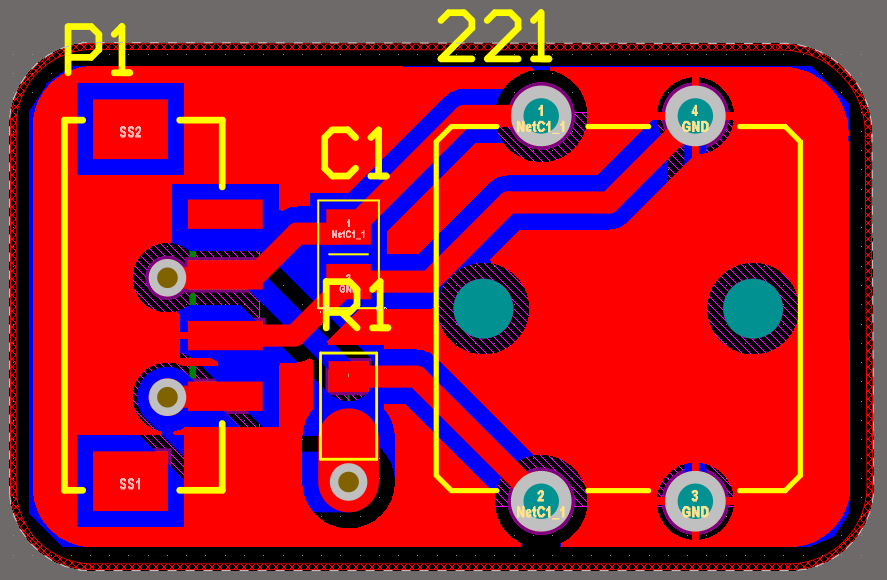
\includegraphics[width=\textwidth]{graphics/ex4/f2.png}
        \caption*{Top Layer}
    \end{subfigure}
    \hfill
    % Ảnh phải
    \begin{subfigure}{0.495\textwidth}
        \centering
        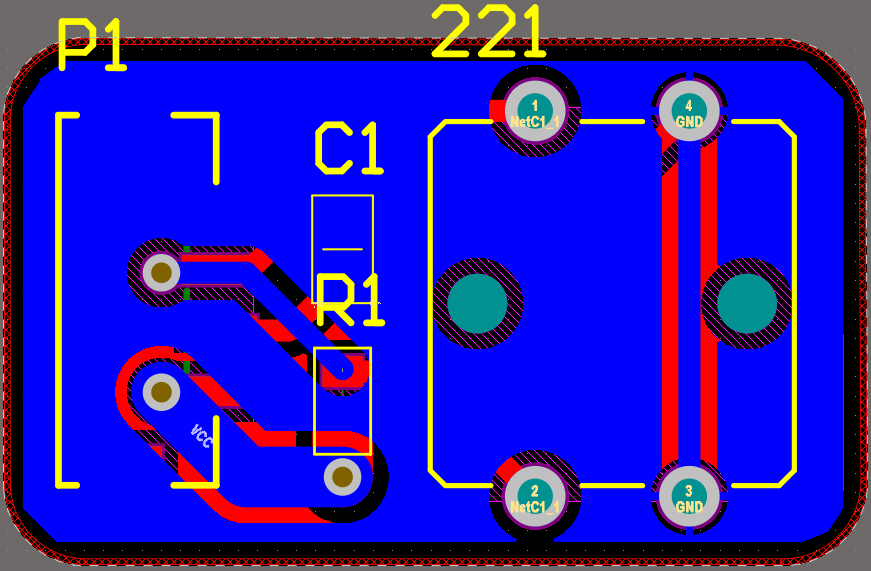
\includegraphics[width=\textwidth]{graphics/ex4/f3.png}
        \caption*{Bottom Layer}
    \end{subfigure}
\end{figure}
\newpage
\textbf{Some 3D views of the PCB:}
\begin{figure}[h!]
    \centering
    % Ảnh trái
    \begin{subfigure}{0.495\textwidth}
        \centering
        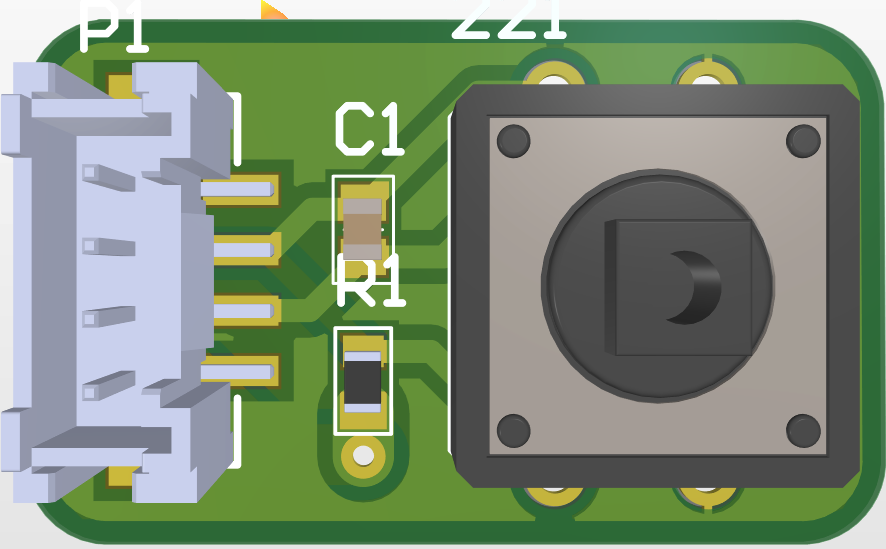
\includegraphics[width=0.95\textwidth]{graphics/ex4/f4.png}
        \caption*{Top view}
    \end{subfigure}
    \hfill
    % Ảnh phải
    \begin{subfigure}{0.495\textwidth}
        \centering
        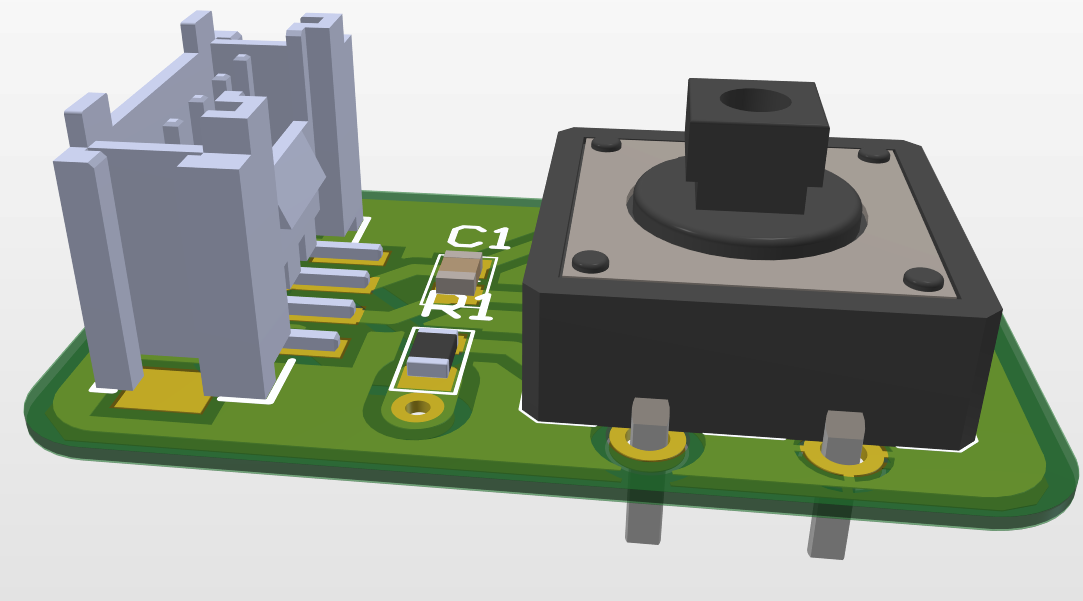
\includegraphics[width=\textwidth]{graphics/ex4/f5.png}
        \caption*{Beside view}
    \end{subfigure}
\end{figure}

\subsection{ADC Input}
\subsubsection{Schematic design}
\textbf{Your image goes here:}
\begin{figure}[h!]
    \centering
    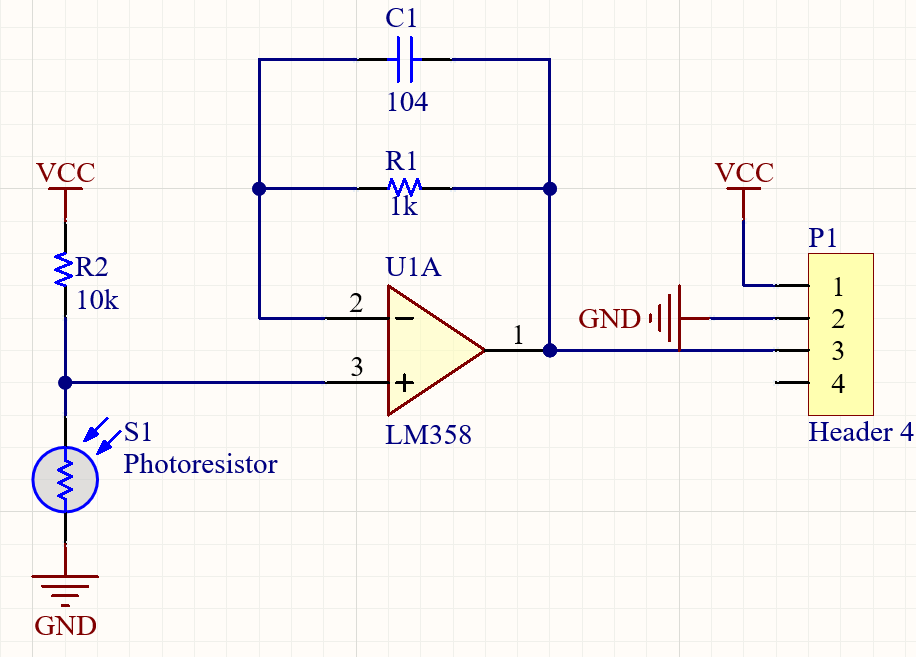
\includegraphics[width=0.9\textwidth]{graphics/ex4/f6.png}
\end{figure}
\newpage
\subsubsection{PCB layout}
\textbf{Your images go here:}
\begin{figure}[h!]
    \centering
    % Ảnh trái
    \begin{subfigure}{0.495\textwidth}
        \centering
        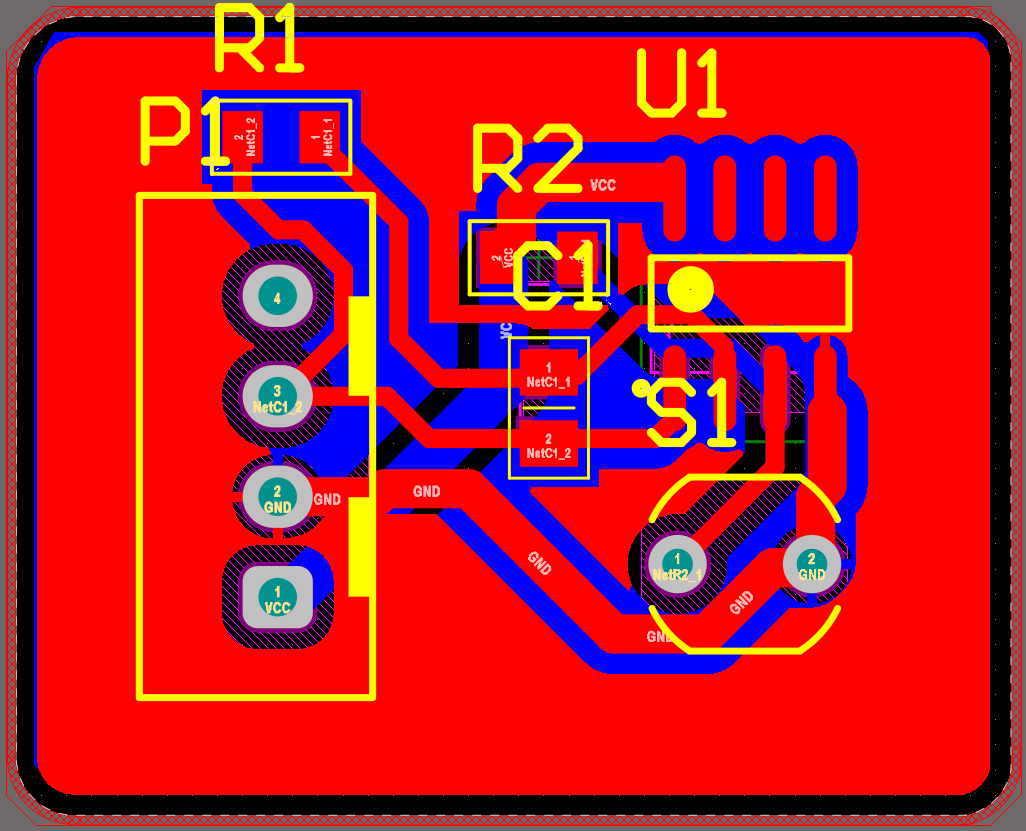
\includegraphics[width=\textwidth]{graphics/ex4/f7.png}
        \caption*{Top Layer}
    \end{subfigure}
    \hfill
    % Ảnh phải
    \begin{subfigure}{0.495\textwidth}
        \centering
        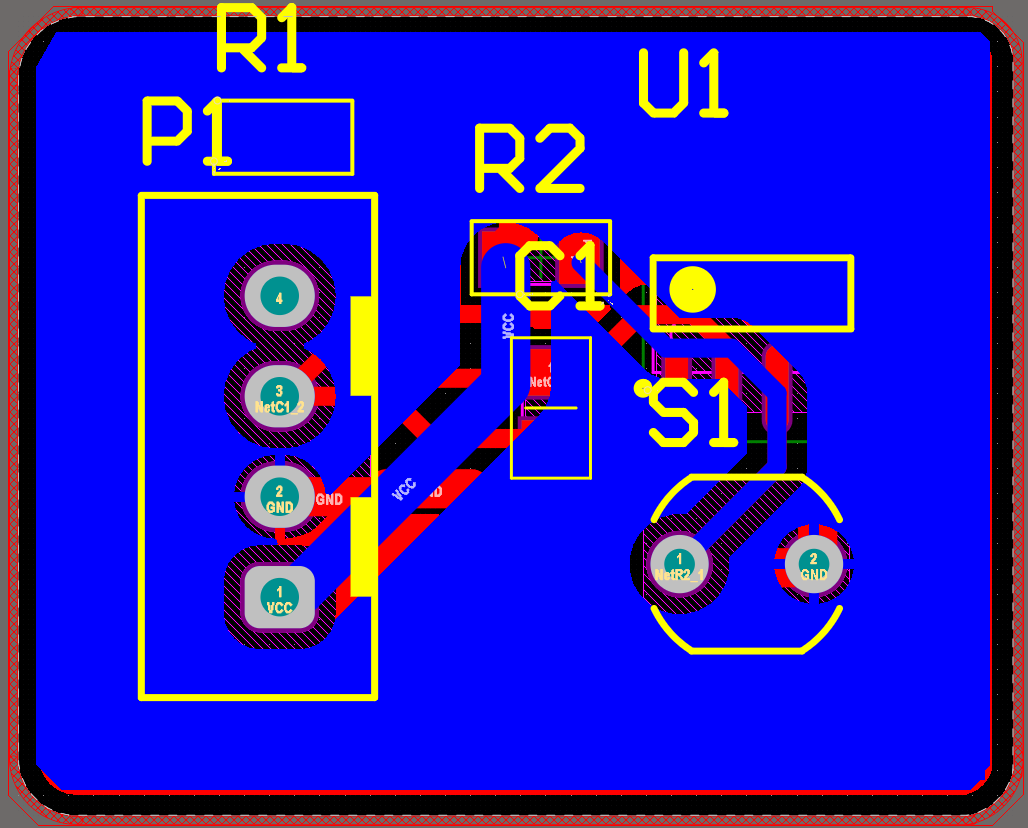
\includegraphics[width=\textwidth]{graphics/ex4/f8.png}
        \caption*{Bottom Layer}
    \end{subfigure}
\end{figure}

\textbf{Some 3D views of the PCB:}
\begin{figure}[h!]
    \centering
    % Ảnh trái
    \begin{subfigure}{0.495\textwidth}
        \centering
        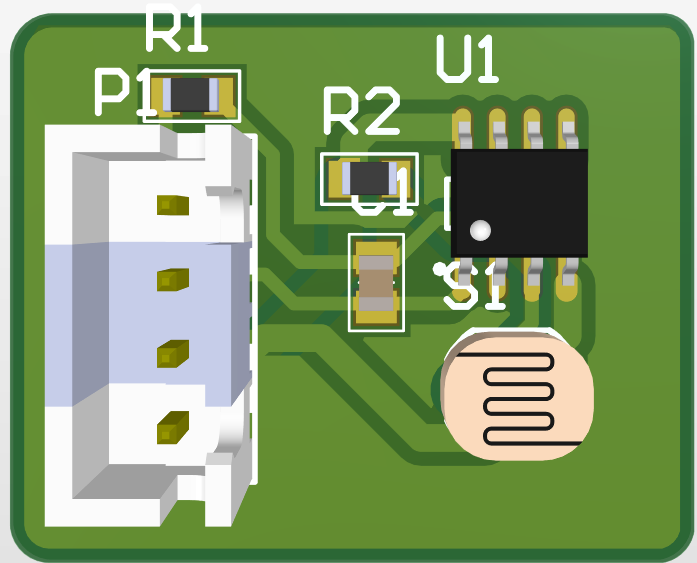
\includegraphics[width=0.95\textwidth]{graphics/ex4/f9.png}
        \caption*{Top view}
    \end{subfigure}
    \hfill
    % Ảnh phải
    \begin{subfigure}{0.495\textwidth}
        \centering
        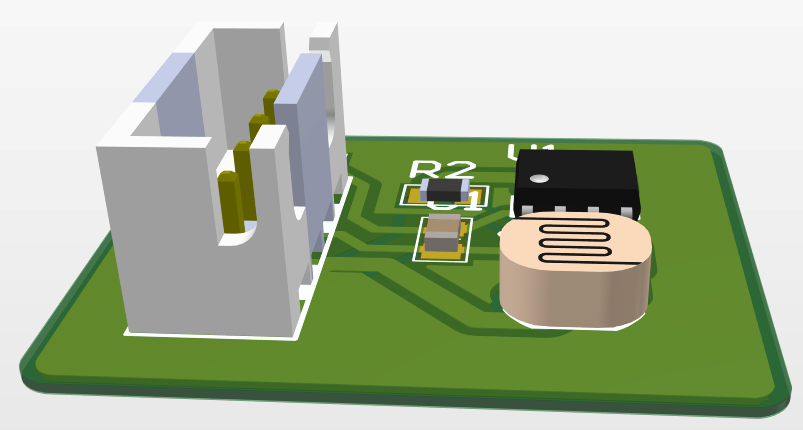
\includegraphics[width=\textwidth]{graphics/ex4/f10.png}
        \caption*{Beside view}
    \end{subfigure}
\end{figure}